\documentclass[letterpaper,twocolumn,10pt]{article}
\usepackage{epsfig,endnotes}
\usepackage{listings}
%% Language and font encodings
\usepackage[english]{babel}
\usepackage[utf8x]{inputenc}
\usepackage[T1]{fontenc}
\usepackage{tikz}
\usepackage{wrapfig}

%% Useful packages
\usepackage{amsmath}
\usepackage{cite}
\usepackage{url}
\usepackage{graphicx}
\usepackage[colorinlistoftodos]{todonotes}
\usepackage[colorlinks=true, allcolors=blue]{hyperref}

\title{\Large \bf Security Project: Fuzzing and Symbolically Executing Cryptographic Implementations}
\date{}
\author{\rm{Heman\ Gandhi} Rutgers University}

\begin{document}

\bibliographystyle{unsrt}

\maketitle

\begin{abstract}
Many programs assume that they implement the common secure encryptions
protocols such as RSA and AES. However, it is difficult for implementors
to test their beliefs: many implementations of the algorithms can be faulty.
This can have untold consequences for users of the implementations.

Fuzzing is a great tool for finding the older exploits that used to wreak
havoc: fuzzers can find buffer overflows and various other attacks dotting
large low-level code bases.

Fuzzing to solve the security holes in encryption programs is difficult, however.
The issues occur over a small fraction of the cases, unlike buffer overflows.
To make the two approaches more compatible, symbolic execution might be able to
constraint the test-case generation to produce tests that are more likely to trip
up cryptographic applications. Another source of difficulty is the reliance on randomness.

This work hopes to detail some approaches and difficulties in using fuzzing to solve
the aforementioned security holes.

This implementation is available at \href{https://github.com/hemangandhi/comp-sec-final-project}{this GitHub.}
\end{abstract}

\section{Introduction}

Fuzzing can be implemented in various ways though the canonical choice
is AFL \cite{AFL}. As the site suggests, fuzzing is a strong way to find
bugs in many low-level programs.

In addition to buffer overflows and side channel attacks, in the last
few decades, the security of cryptography has been called into question.
\cite{miningPQ} However, to test such implementations, such as the entropy
of random number generators, fuzzing does not suffice.

Here, a middle ground is explored and simpler alternatives are analysed.
While initially thought to be the simplest direct approach, fuzzing Java
informed by symbolic execution turns out to be overly complicated. It
may be simpler to statically generate the test cases. This is discussed in
the later sections: section 2 details the background on fuzzing, symbolic
execution, and how their union would test the security of cryptographic
code; section 3 details the experimental set up with JFP, SymExe, and badger;
section 4 discusses an alternate approach that may be simpler for initially
using symbolic execution; section 5 concludes.

\section{Related Works}

There are a two classes of related works: works on fuzzing, and works on breaking
cryptographic protocols. Finally, there is also their meet: works on fuzzing against
cryptographic code.

\subsection{Fuzzing and Symbolic Execution}

Fuzzing is a simple technique at its core: it is
to generate test cases and run the program until
the program fails. This, however, is difficult to
reason about for various reasons. The generation of
inputs is the biggest concern: it is very difficult to
generate test cases that cover some black-boxed executable.
Various approaches are discussed here.

First, there is the classical AFL approach. \cite{AFL}
is the conventional fuzzer used by many to test low-level
libraries. On its site is a large trophy case of bugs found
by the genetic algorithm at the heart of this fuzzer. The algorithm
tracks coverage by labelling basic blocks and then using the xor
of the blocks to maintain the edge between them. The collection
of edges forms a fairly unique representation of an execution trace.
If an execution trace does not lead to a new behavior, the test case
is not further explored. Otherwise, if new behavior is found, the genetic
algorithm is used to further explore the input.

Another approach is to compare two runs of the program at a higher
level. This approach is useful for finding side-channels. Fuzzers
for this have been shown to be effective \cite{diffFuzz} \cite{cdf}.
Here, \cite{cdf} concludes that various Go, Python, and C++ libraries
do not insure users against poor parameter choices and sometimes do not
fully adhere to standards.

The two approaches above are powerful, however, here, symbolic execution
is explored. Symbolic execution would allow the fuzzer to powerfully reason
about number theoretic invariants in the various cryptographic algorithms
implemented. This has not been done directly. Indirectly, much tooling is
provided. In particular, \cite{badger} runs a trinity of processes to fuzz
Java code. There is a fuzzer and a symbolic executor. These are joined in
badger itself that uses the symbolic executor to inform the fuzzer to better
test and execute Java. Simply: the symbolic executor finds program paths
and the conditions that would cause the path to be executed. This is put
into a trie and the leaf nodes are added to a queue. A leaf is dequeued,
turned into a test case (by any SAT-solver) and that test case is passed
to the fuzzer.

Hence, the fuzzing is an active field with various applications to testing
cryptographic code.

\subsection{Cryptographic Algorithms}

Cryptographic algorithms power the modern internet. Many implementations
of varied algorithms are used to secure many layers of the OSI stack: routers
sign off their identity, servers do the same with SSL and TLS, and at the message
and application layer, HTTPS encrypts the messages.

RSA is a common algorithm that is widely popular. For security, however, it depends
on large primes. Furthermore, in the internet, it needs that all the primes found
are independently found. For instance, if a server uses $P$ and $Q$ and another
server uses $Q$ and $R$, and all three, on their own are secure, there is still a
vulnerability. Namely, if an attacker knows this about the server, they can quickly
compute $gcd(PQ, QR)$ ($PQ$ and $QR$ being public as a part of RSA). This would give
the attacker $Q$ from where finding $P$ and $R$ is a matter of division. This issue
can be endemic to a server, if the random number generator is poor enough. This is
a widespread issue, as found in \cite{miningPQ}. A fuzzer could be informed by their
work and resources to ensure that primes used are most likely not vulnerable to this
$gcd$ attack.

This is suggestive of various invariants and issues that may occur in implementations.
For this work, only RSA and the entropy of random number generators are considered.
These should be a good starting point in a lengthier investigation of cryptographic
algorithms.

\subsection{The Union of the Approaches}

As suggested above, differential fuzzing has proven useful for revealing side-channels
and even found bugs in cryptography libraries \cite{cdf}. That said, there is a bigger
discussion of symbolic execution used to verify cryptography.

In fact, network protocols can be tested through symbolic execution \cite{symExeCrypto}.
Here, it is also possible to statically detect the use of bad pseudo-random number generators.

This work is an attempt to extend this fledgling field. Here, it is established that badger's
architecture \cite{badger}, is too complex for quickly investigating whether symbolic execution
is feasible -- a more foundational approach would be more suitable.

\section{The Program}

Here, the structure and the necessary changes to badger are documented. Due to the complexity
of the changes two things were impossible: searching using SymExe for the correct invariants,
and foundationally building up a set of searches and paths that could find problems with
cryptography implementations.

As an initial test, a publicly provided RSA was used \cite{RSAImpl}. It is documented
that if $message \geq modulus$ or $gcd(\phi, pq) \neq 1$, the encryption fails. The
hope was to extend badger so that these two bugs and possibly a bad pseudo-random
number generator could be detected.

\subsection{The Architecture of Badger}

Badger is a behemoth. It runs a trinity of rather large Java libraries. A dependency graph is likely the best
description:

\begin{wrapfigure}{l}{5cm}
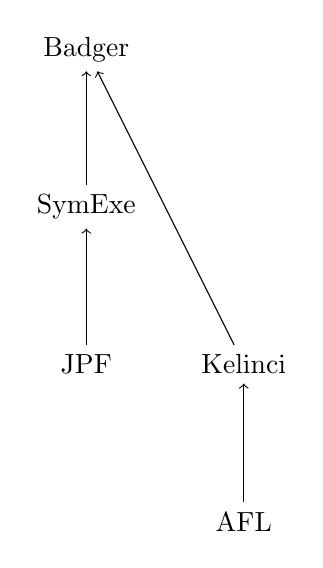
\begin{tikzpicture}[node distance = 2cm, auto]
\node (B) {Badger};
\node (S) [below of=B] {SymExe};
\node (J) [below of=S] {JPF};
\node (K) [below of=B, right of=S] {Kelinci};
\node (A) [below of=K, right of=J] {AFL};
\draw[->] (S) to node {} (B);
\draw[->] (K) to node {} (B);
\draw[->] (A) to node {} (K);
\draw[->] (J) to node {} (S);
\end{tikzpicture}
\caption{The badger trinity and dependencies}
\end{wrapfigure}

Badger orchestrates the two large Java libraries to symbolically learn the unexplored paths in a program and
then fuzz them through Kelinci (a Java AFL wrapper). This work focusses on the SymExe and JPF side, in hoped
to statically detect the use of bad pseudo-random generators and then perhaps adjust the SymExe searches to
explore invariants in cryptographic code.

Below, the JPF property added is mentioned with a few potential extensions. Then the infeasibility of extending
SymExe is mentioned. (Note that SymExe is a part of badger, not a library.)

\subsection{Extending JPF}

The first work was to extend JPF to ensure that all random generators used were secure. This was not done too
thoroughly for a first implementation: JPF provides properties that are checked at every step of their VM's execution.
Using this, another property was created to check that \texttt{Math.random} and \texttt{java.util.Random} were not
used (both are known to be insecure). The property queries the call stack and ensures that no
methods in \texttt{java.util.Random} are not called by checking that the class the method executing is in is not \texttt{java.util.Random}.
Similarly, the property asks the call stack if it has entered \texttt{Math.random}.

However, JPF does not provide enough of a native interface to emulate \texttt{java.security.SecureRandom}. The
file creation fails since it is impossible to emulate \texttt{/dev/random} purely symbolically. This would have to
be added.

\subsection{SymExe Searches}

SymExe performs searches by expanding a trie of potential execution paths. Nodes that are high and are at branch points
are, by the default metric, considered the most worth exploring.

Depending on the cryptographic algorithm in mind, SymExe could be extended to also create more paths based on the numbers
processed: the numbers sharing common factors would be one of the potential paths, for instance. This would cover one of the
bugs mentioned in the source code \cite{RSAImpl}.

However, this approach does not generalise as most of the paths would depend on random numbers that were generated elsewhere.
Hence, one would have to consider these cases and accurately model randomness.

\subsection{Takeaways}

The biggest lesson is perhaps a change in approach. Java is rather clunky by design and the dependency tree is quite deep
for initial experimentation. A couple approaches would be a more feasible starting point:
\begin{itemize}
    \item Instrumenting a C AST for AFL to fuzz cryptographic code.
    \item Using a lighter symbolic executor to merely generate the path conditions (as a proof-of-concept).
    \item Using more broken implementations or simpler sub-parts of algorithms for testing.
\end{itemize}

Either of these can also be pursued in a simpler language like C, where the security of the randomness generator
cannot be obfuscated by sub-classing or other complicated structures.

Additionally, the approach has limited visibility into the workings of \texttt{BigInteger} which is used in Java
to compute with large numbers. C would be a better alternative for this as these implementations would be easier
to target.

Finally, an important thought is that randomness is very difficult to emulate. Without much external information,
it is difficult to guess the entropy of random numbers. For symbolic execution, it may be necessary to treat
a random number as an input fully controllable by the symbolic executor, but it would be more informative to
propagate probabilities and similar details (see the potential future work below).

\section{Future Work}

There are many ways -- in addition to the ``short-term'' takeaways above that could apply to cryptographic algorithms.
These would be large projects predicated on the success of the symbolic execution fuzzing approach. These also bring up
questions about cryptographic algorithms and how general any such system can be.

The two systems conceived of below are more static analysis extensions for fuzzing cryptographic algorithms.

\subsection{Generally Specifying Algorithms}

Technically, an implementation should be a specification of an algorithm. Of course, the reason such work is pursued,
is that implementations often are not completely correct.

However, in order to test an implementation of a number theory algorithm, some external information might be necessary.
Automatically inferring that a user may be able to solve for the public key, per say, would not be productive.
Hence, some system of annotations should be considered so that a static analysis would know how an attacker would be
approaching a particular implementation.

This can be done through a DSL that generates the input. Such an approach has proven to be effective in \cite{singularity}
for finding worst-case run times of various algorithms. A similar idea may extend to fuzzing cryptographic algorithms
are a DSL can specify the conditions that would favor an attacker and these can be fed to the program to see if it is
vulnerable. Naturally, such a DSL would also specify what parameters are publicly knowable and what parameters are intended
to be kept secret.

\subsection{Symbolic Randomness and Propagating Entropy}

Another part of statically determining the security of an implementation is to have the entropy of random number generators
known to the static analysis tool. As the random numbers are used in an algorithm, the entropy can be tracked -- through
static analysis or symbolic execution (if not both). This would allow tools to be aware of how random a given generator
is.

This could tie with the above where the DSL may specify a minimum randomness in the output it seeks. Then executions can
fuzz by concretely executing the program and also symbolically track the entropy. Either failing would then be considered
a failure of the code.

Such an approach would be supplemented by probabilistic programming. This is detailed in \cite{probProg} where various
applications are discussed. Generally, such programming is used to discuss distributions and contain them as first
class objects -- so that sampling and reasoning about said sampling are made simpler. These languages are a great
model for propagation of entropy and the other arguments above.

\section{References}

\bibliography{sample}

\end{document}
